\section{Knowledge Graph based MMM Product Search Dataset}

In this section, we introduce the KG based MMM\footnote{MMM (anonymized for blind review) is a major e-commerce platform in China.} Product Search dataset. We first introduce the background of releasing such a dataset and then introduce the construction of this dataset.

\subsection{Dataset Background}

Different from other e-commerce platforms like Amazon, Taobao, JD etc., MMM is a life-service e-commerce platform focusing on retailing of services and retailing of products. As a life-service e-commerce platform, it is closely related to people's daily life and is gradually becoming ``the largest convenience store in China''. In the ``Top 100 List'' of China's e-commerce in 2021, MMM ranked second with a total company value of 1,128.357 billion yuan, second only to Alibaba. Figure \ref{fig:meituan} is the user interface of MMM APP and its services include takeaway, vegetables, fruits, products in supermarkets and convenience stores, flowers, medicines and any other products that we can see in our daily life. Various kinds of products make PSR task in our secnario more challenging. Besides, as life-related products is closely related to people's daily life, one product can have a lot of synonyms, which adds more difficulty to PSR task. Thus, external knowledge is especially necessary for this task in our scenario. Against this background, we construct and release a PSR dataset with KG. 

\begin{figure}[th] \centering
    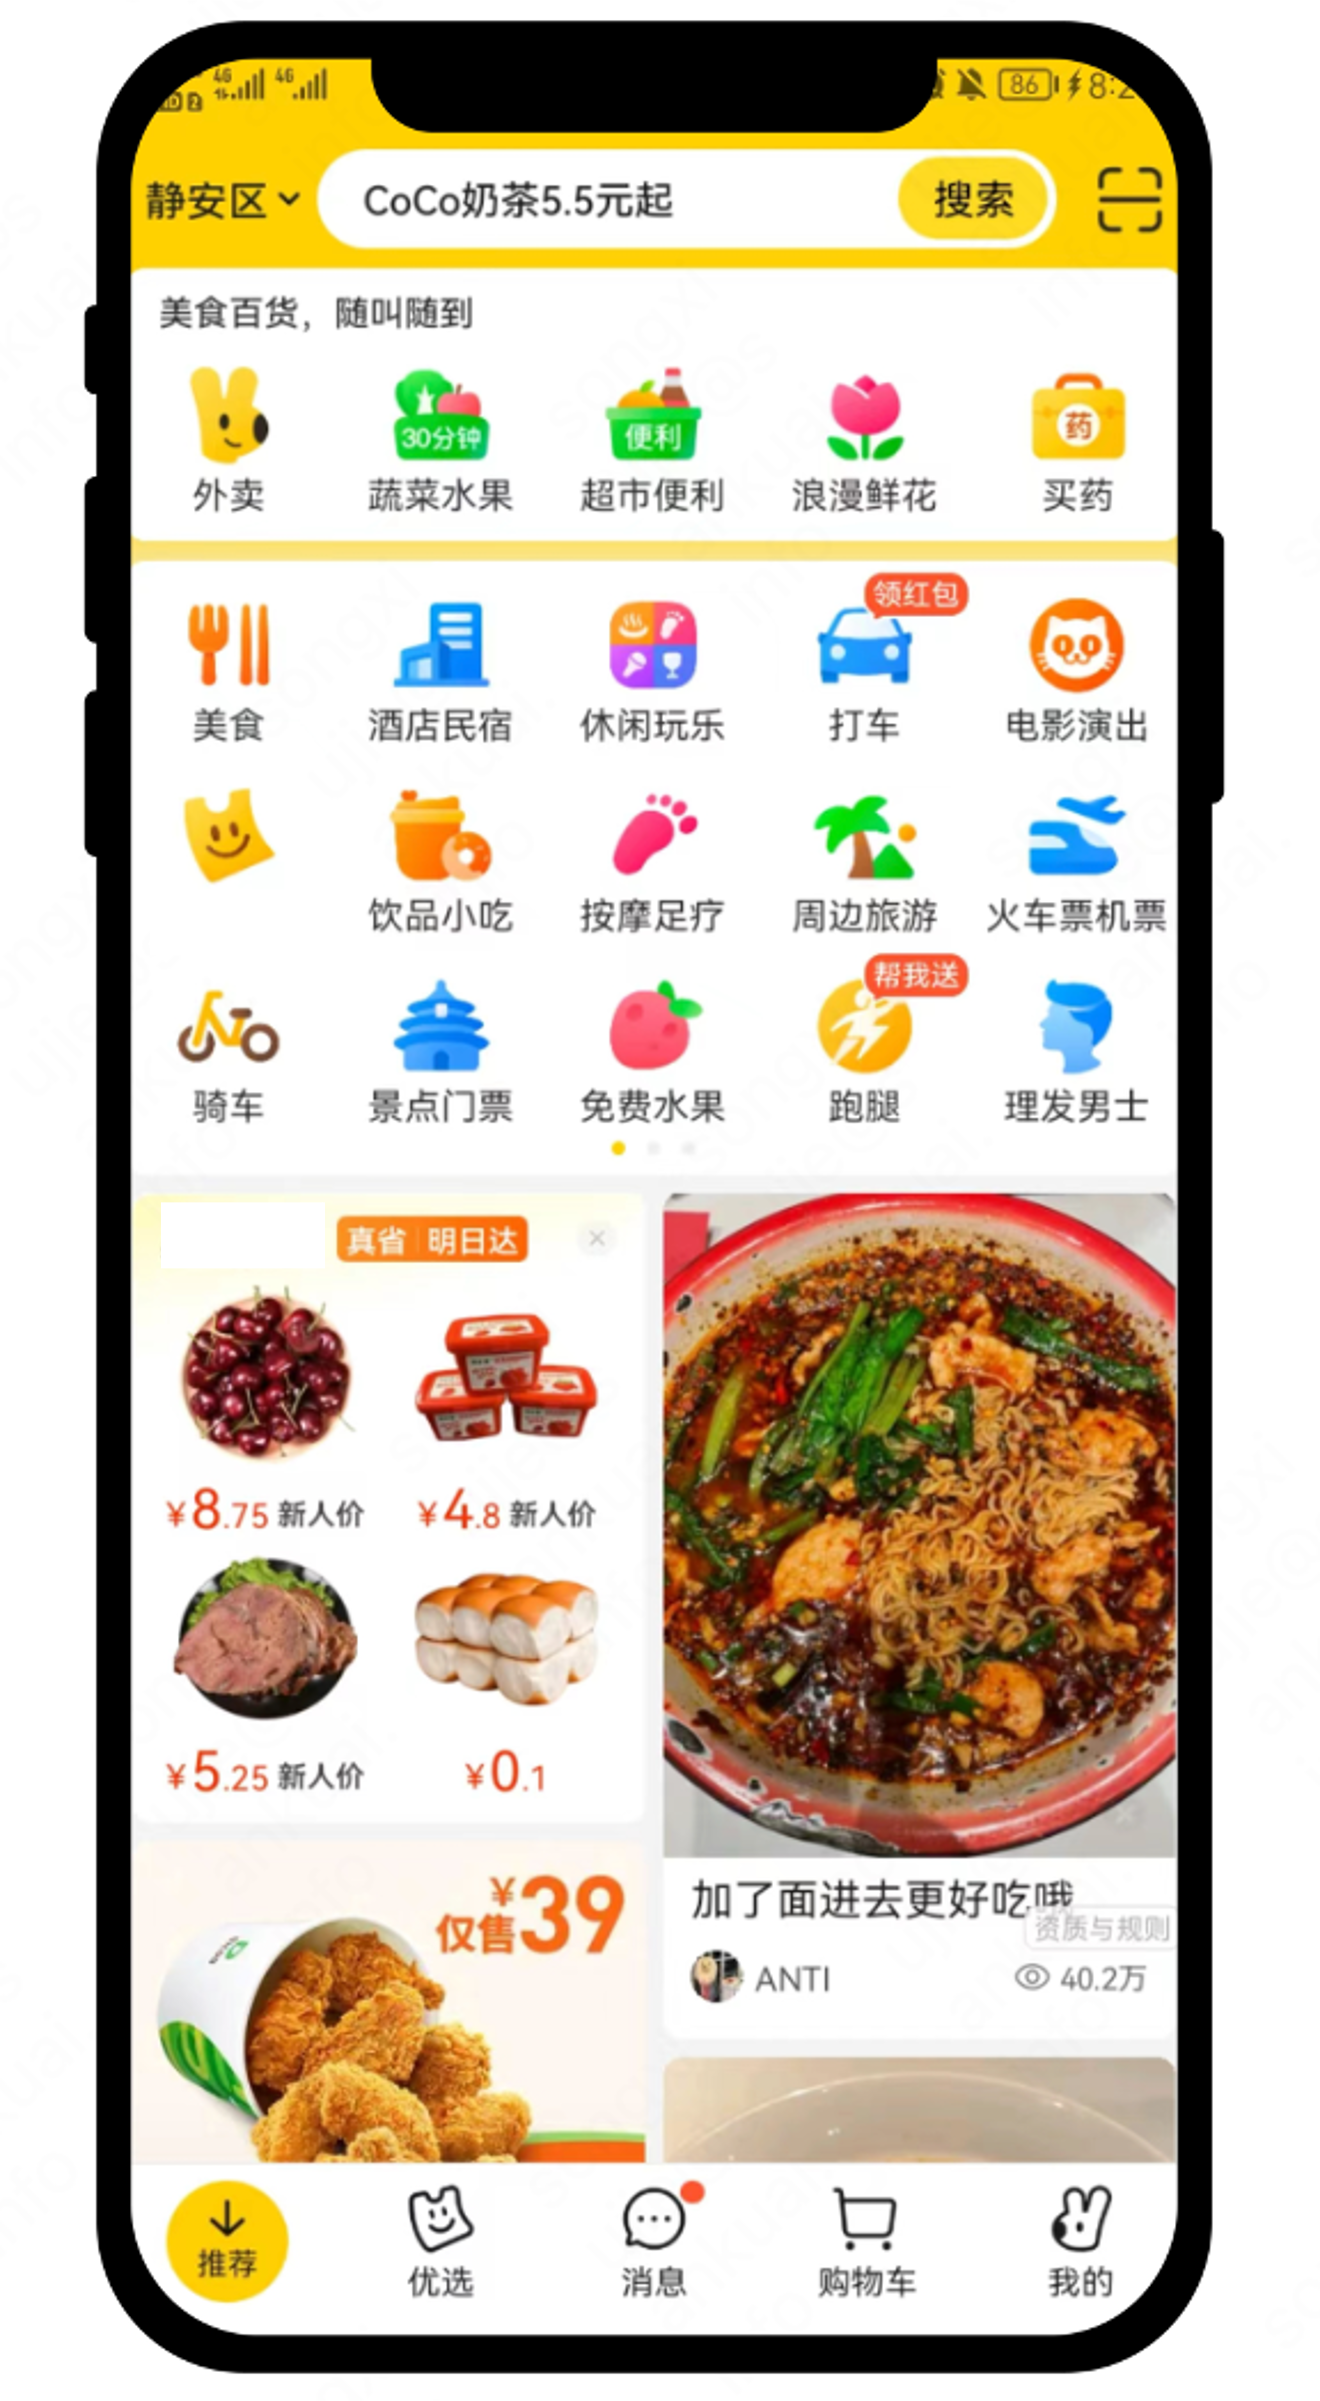
\includegraphics[width=0.23\textwidth]{meituan_app}
    \caption{User interface of MMM.}
    \label{fig:meituan}
\end{figure}

\subsection{Dataset Construction}

To evaluate the performance of PSR models with KG, especially in life-service scenario with various product expressions, we construct a challenging dataset called MMM Product Search (MMMPS) from our real business logs. 

Firstly, we collect <query, product> pairs with their exposure frequency from search logs. To alleviate noisy logs, we filter the queries using a query corpus that auto-collected from logs and product titles with NER. Queries appear in query corpus will be kept and queries do not appear in the corpus will be dropped. Note that, the size of the query corpus is much larger than the size of the concept graph. Then, we randomly sample a subset of pairs by their exposure frequency to ensure pairs with both head and tail frequencies are maintained. To further focus on the hard scenarios, we use a group of models to validate these sampled pairs and sample a hard dataset from different buckets with different consistency scores or average validation scores to ensure both easy and hard pairs are sampled. Finally, we recruit experienced annotators to manually label the dataset. Data groups with over 95\% accuracy in quality checking are used in our final dataset. 

Apart from the label of <query, product> pair, we also provide a subset of the concept graph associated with queries and a subset of the hierarchical category taxonomy associated with products. The concept graph is a fine-grained knowledge graph that contains hypernym and synonym relations among concepts, e.g. ``murphy'' is a synonym of ``potato''. The hierarchical category graph is a coarse-grained KG that contains three level categories, e.g. ``Vegetable / Rhizomes / Potato''. Figure \ref{fig:taxonomy} shows a fragment of our three-level tree-structured taxonomy. Note that although both KGs have been reviewed by annotators to ensure the quality, noisy data cannot be completely avoided, and that is the real scenario we are facing.
% \zelin{maybe we should detail the two graphs? they are the key components in this dataset}

\begin{figure}[th] \centering
    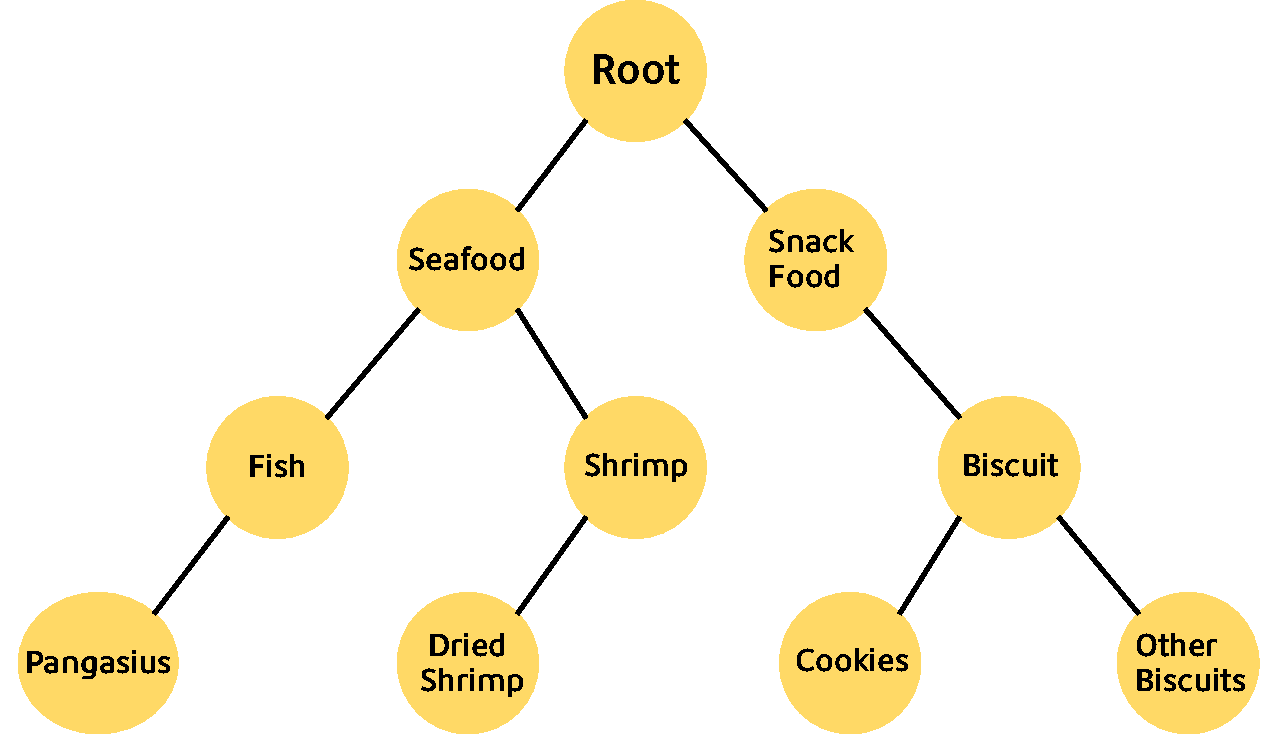
\includegraphics[width=0.4\textwidth]{taxonomy}
    \caption{A Fragment of Taxonomy.}
    \label{fig:taxonomy}
\end{figure}

% \sansa{\sout{maybe you can mention that this dataset is in Chinese but I prefer not to use Chinese in the main body of paper}}

% we do 10-fold cross-validation by our baseline model and randomly sample a hard dataset by their validation score to ensure both easy and hard pairs are maintained. 

% ``\begin{CJK}{UTF8}{gbsn}土豆/根茎类/蔬菜\end{CJK}''

% \begin{CJK}{UTF8}{gbsn}马铃薯\end{CJK}
% \begin{CJK}{UTF8}{gbsn}土豆\end{CJK}